% Chapter 1

\chapter{Experimental Results} % Main chapter title

\lhead{Chapter 5. \emph{Experimental Result}} % This is for the header on each page - perhaps a shortened title

%----------------------------------------------------------------------------------------
In this chapter, we first give an overview of the visual and social 
feature vectors constructed and then we discuss the classifiers 
tested. In end, we describe the results on four benchmark data-sets.

\section{Feature Vectors}
We extracted the five image features SIFT, GIST, HOG-LBP, CIELAB 
color space vector and GLCM as described in the previous chapter \ref{FeatureExtraction}
Apart from these visual features, we constructed two feature vectors on the basis of social meta data. These feature vectors are 
constructed after doing analysis of social data and obtaining a binary feature vector, indicating the presence or absence of a 
social/textual element for the image.This high dimensional binary vector lead to two different feature 
vectors. First, where dimensionality reduction was done by Latent Semantic Indexing and the second,  where dimensionality reduction was  by Random Projections.
%----------------------------------------------------------------------------------------

\section{Classifiers Used}
After experimenting with various classifiers like Random Forest, MLP 
(Multi Layer Perceptron), libSVM (with various kernels linear, RBF, 
$\chi^2$, histogram intersection), we found that in case of 
image features libSVM with $\chi^2$ kernel worked best and in case of 
social features libSVM with the linear kernel gave us the best 
results. We,therefore, used libSVM with $\chi^2$ kernel as the classifier 
for visual feature vectors and libSVM with Linear Kernel as the
classifier for social feature vectors.


\section{Classification Results}

In the following part of this chapter, we have shown classification results on various labels of four data sets as mentioned in \ref{Chapter3} .

The results are divided in four subsections according to the four data-sets. First, we have shown  the classification results from all the features  extracted. We first experimented with the classifiers based on individual features, means separate classifier from SIFT, HoG, 
GIST , GLCM, COLOR, social Features generated through LSI and social Features generated through LSI. In next step, we did ensemble of classifiers obtained by different image and social meta data classifiers to learn the linear combination of weighted classifier.
%{\bf *** Above not clear. What do you mean by ensembling features? Normally, one ensembles classifiers. Rewrite the above. ***}

We have also given qualitative and quantitative conclusions/observations  of our results. We have shown a comparison with published results  on each of these four benchmarks or with results in associated competitions. 

The goal of all these comparisons is to assess the improvement that can be obtained by using social meta-data for images. We reported the mean average precision (MAP) for the sake of comparison with published materials and competition results. We also gave the accuracy for the binary prediction/classification of labels.

All these results are for tenfold cross validation. For ensemble methods, we divided the data in three parts: training, testing and validation. We randomly chose 10\% instances for validation set and learned weights for the linear combination of the classifiers, which provided best results. After learning these weights, we used the optimized combination of the classifiers to do testing on test set.

For better visualization, we have broken our result in three tables, for each data set.
\begin{itemize}
\item In first table, we have shown results using only the image descriptors. In this table, we have only considered the visual features and shown the classification result for each of extracted visual feature.
\item In second table, we have shown results using only the social meta-data descriptors. In this table, we have only considered the social meta-data features . We have shown the classification result for each of the method LSI and Random Projections.
\item In third table, we have compared result with the published paper. In this comparison, we have taken the result of the ensemble of social and visual classifiers, and best of visual and best of social descriptor 
\end{itemize}

We have created such tables for comparing mean average precision and accuracy for each of the data-set.

\subsection{MIR Flickr collection }
%----------------------------------------------------------------------------------------
MIR has high quality photographic images. It has rich meta data attached with it. This provides a wide variety of image retrieval bench-marking scenarios.

In \citep{MIRresults}, a combination of social data and low-level content-based descriptors improve the accuracy of visual concept 
classifiers. We use the results of this paper as a comparison metric for our results.

In \citep{MIRresults}, they have used the following four sets of image features:
\begin{itemize}
\item HMMD Color Histogram descriptor.
\item Spatial Color Mode descriptor.
\item MPEG-7 Edge Histogram
\item MPEG-7 Homogeneous Texture descriptor
\end{itemize}

Apart for these low-level content based descriptors, they also used flickr tags of visual concepts.  A set consisting of 293 binary features was developed using these tags. These tags were chosen such that every tag corresponds with at least 50 images in the MIR Flickr collection.

They have used two classifiers one is Linear Discriminant Analysis  and other is support vector machines. For each of these classifier, they have first tested with classifier using only the image descriptors and then they tested using the image desciptors $+$ Flickr tags as features. The classifiers were trained on the 24 potential labels, and 14 regular (subjective) annotations. We chose the results of the labels, we have considered. We could not cover all the labels because for other labels, we could not get much data on flickr. That data might be available at that time but now those image URLs are either denying access or do not exist. So, we refrain our self to a subset of those 38 labels.

We have compared the classification accuracy and mean average precision between  classifiers based on low-level features only and classifiers that additionally use the Flickr tags as features.
We have shown our result in following tables. 


\begin{itemize}
\item In table \ref{MIRPrecisionVisual}, we have shown accuracy using only the image descriptors. In this table, we have only considered the visual features and shown the classification result for each of extracted visual feature.
\item In table \ref{MIRPrecisionSocialFeatures}, we have shown accuracy using only the social meta-data descriptors. In this table, we have only considered the social meta-data features . We have shown the classification result for each of the method visual feature, LSI and Random Projections.
\item In table \ref{MIRPrecisionOverAll}, we have compared our accuracy with the published paper. In this comparison, we have taken the result of the ensemble of social and visual classifiers, and best of visual and best of social descriptor. We have divided the result of \citep{MIRresults} in two parts. One is for SVM Classifier and second is for LDA Classifier. Each of this has two sub parts, one is for only the image descriptors and second sub part is for combined descriptor of image and flicker tags.

\item In table \ref{MIRAccuracyVisual}, we have shown mean average precision using only the image descriptors. In this table, we have only considered the visual features and shown the classification result for each of extracted visual feature.
\item In table \ref{MIRAccuracySocialFeatures}, we have shown mean average precision using only the social meta-data descriptors. In this table, we have only considered the social meta-data features . We have shown the classification result for each of the method visual feature, LSI and Random Projections.
\item In table \ref{MIRAccuracyOverAll}, we have compared our mean average precision with the published paper. In this comparison, we have taken the result of the ensemble of social and visual classifiers, and best of visual and best of social descriptor. 
\end{itemize}

\subsubsection*{Observations}
\begin{itemize}
\item The classifications based on visual only features gave an 
average precision of 76.15\%, which outperformed the low level image 
descriptor based classification with 40.43\% in case of LDA and 
44.38\% in case of SVM. The result was also better than 
classification based on the combination of low level image 
descriptors and Flickr tags. Here we saw a precision increment of 
28\% as compared to SVM results in paper and 26.40\% as compared to 
LDA results in paper. This result is an indication that our choice of image descriptors gives a better semantic analysis of image then the low level image descriptors used in image.

%{\bf *** The table of results is confusing. You must clarify the following:
%- What image descriptors are in use in cols 4 and 6? Do you mean the 4
%descriptors you enumerated earlier?\\
%----I have broken the table in three parts, it is more comprensible now.-----

%- What does addition of Flickr tags mean? Are you processing them in any
%way before adding them or is it just bag-of-words or tfidf or what?\\
%----I have added a description for the processing done in published paper. See the intial part of this subsection-----


%- I assume the columns for SIFT GIST etc. are values when only that
%feature is used. Have you tried combining them into a single vector and see
%what you get? 
%----I have not done this part. But I will do this before FINAL SUBMISSION. -------

%In your feature extraction chapter you seemed to imply that  your vector contained all the features. Alternately, have you tried
%ensembling just the various visual features - example majority vote?\\
%----I have not done this part. But I will do this before FINAL SUBMISSION. -------

%- Unless you try the various ways available to improve accuracy from 
%just the visual features it would be wrong to claim improvement by 
%adding social meta tags.\\
%----I have not done this part. But I will do this before FINAL SUBMISSION. -------

%- Does your ensemble method mean visual features + social meta tags? If yes
%which one of LSI or RP are you using? Or are you using both?\\
%---In ensemble, we are learning weights for the linear combination of the classifiers. We considered all the five classifiers obtained from image desciptors and two classifiers (LS and RP) obtianed from social descriptors. Described this in the intial of classification result section.

%- I think there is a need to describe each column in your table precisely.
% You must say exactly what features were used and what classification 
% technique was used. It may a better idea to split the single large table
%into multiple smaller tables. For example, you can have separate tables for
%purely visual features and purely social meta tags. Then you can have a
%third table where you take the best values from the previous two and
%compare with visual+social at the feature level (that is combine features
%and have a single classifier) and via ensembling where you have separate
% classifiers for visual and social features. ***}
%-Done That

\item When we do classification on the basis of social features 
computed using LSI, we got an average precision of 87.59\%. This was 
39.71\% more compared to SVM classification of combined features of 
Flickr tags and low level image descriptors and  37.83\% more 
compared to LDA classification of this combined feature set. This might be because we covered more tags and sources of meta-data then the taken by the paper.

\item LSI based social feature classification outperformsed our visual 
only classification with 11.43\% precision increment.  It shows a 
precision gain of 51.86\% and 55.81\% on the low level image 
descriptor based SVM classification and LDA classification respectively.

\item Ensemble of the social features and visual features provides 
average precision of 90.58\% which is 40.83\% more compared 
published result and 2.99\% more compared to LSI method.

\item This 42.70\% precision gain compared to published result is 
consistent with the results shown in \citet{Jure}. They obtained a 
precision gain of 42\% using the social features.

\item Our LSI based method works better for all labels except 
\textit{Clouds}. The images in this label shows better result with HOG\_ LBP features. This is due to low volume of social information attached with the data related to these images. For example, we can see that in \ref{fig:Image MIR Examples}, first image is a non-cloud image and second image is image labeled as cloud. The second image has most of the comments saying nice view, beautiful place etc. Very less textual cues actually indicate the cloud part. Apart from this, these images contains various visual descriptors , which is more emphasized intensity gradients or distributed edge directions. Therefore, HOG-LBP and GLCM features works quite better for this label.

\begin{center}
\begin{figure}
\centering
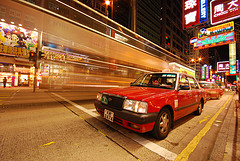
\includegraphics[width=3cm, height=3cm]{./Pictures/MIR/cloud_0.jpg}
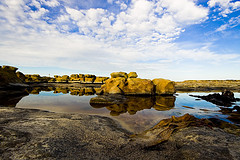
\includegraphics[width=3cm, height=3cm]{./Pictures/MIR/cloud_1.jpg}
\caption{MIR Cloud Examples}
\label{fig:Image MIR Examples}
\end{figure}
\end{center}

%------{\bf *** What is meant by 'high visual concepts entailed'? ***}
%------Answered

\item The results of social features and image features are quite 
close for \textit{night, tree, sea} and \textit{river}. This is the 
result of a great degree of visual information present with these 
images in contrast to social information in comments (or other social 
entities), as they are natural outdoor photographs.

\item The classifications based on visual only features give an 
average accuracy of 76.03\%.
{\bf *** You have not ensembled visual only features. See what you
get when you ensemble visual only features and compare. ***}

\item The classifications based on social only features with LSI pre-
computation give average accuracy of 86.25 outperforming the visual 
features only method with 10.22\%.

\item The ensemble of all the features provide an average accuracy of 
88.80\% outperforming the social feature only accuracy with 2.55\%.

\item GLCM plays an important role in the case of \textit{Bird , male , baby}  labels.

\item GIST plays a pivotal role in case of labels \textit{female, male} and \textit{tree}.
\end{itemize}



%------------------
\begin{table}
\centering
\caption{ MIR Precision Comparison: Only Visual Feature} % title of Table % used for centering table
\vspace*{0.2 cm}
\begin{tabular}{| c | c | c | c | c | c |}
\hline
 {\multirow{2}{*}{Labels}} & \multicolumn{5}{|c|}{Visual Feature Based Classification} \\ 
 \cline{2-6}
 & HOG-LBP & SIFT & GIST & COLOR & GLCM \\  [1ex] \hline
Flower &  78.94 & 41.60 & 73.19 & 70.37 & 64.40 \\  [1ex] \hline
Car & 83.27 & 56.54 & 71.70 & 64.35 & 76.65 \\  [1ex] \hline
Bird &  70.11 & 47.96 & 61.77 & 60.63 & 71.17 \\  [1ex] \hline
Dog &  73.68 & 47.39 & 68.80 & 65.31 & 67.67 \\  [1ex] \hline
Night &  82.40 & 58.00 & 70.40 & 79.16 & 81.37 \\  [1ex] \hline
Tree &  76.92 & 54.59 & 74.97 & 61.64 & 76.11 \\  [1ex] \hline
Clouds &  90.91 & 50.88 & 79.78 & 67.31 & 76.55 \\  [1ex] \hline
Portrait &  69.31 & 50.61 & 65.30 & 59.99 & 65.85 \\  [1ex] \hline
Female & 63.72 & 52.56 & 62.27 & 54.11 & 58.77 \\  [1ex] \hline
Male &  60.16 & 50.62 & 60.96 & 52.88 & 61.79 \\  [1ex] \hline
People &  68.36 & 60.37 & 58.19 & 55.56 & 59.18 \\  [1ex] \hline
Sea & 88.48 & 53.04 & 77.20 & 73.42 & 81.05 \\  [1ex] \hline
River & 77.14 & 46.68 & 69.73 & 68.55 & 71.10 \\  [1ex] \hline
Baby & 77.58 & 47.71 & 72.29 & 73.86 & 80.06 \\  [1ex]  \hline
\end{tabular}
\label{MIRPrecisionVisual} % is used to refer this table in the text
\end{table}
%-------------------
%-----------------
\begin{table}[!ht]
  \caption{ MIR Precision Comparison: Social Features based on LSI and RP Methods} % title of Table % used for centering table
  \centering
  \begin{tabular}{|c|c|c|}
  \hline
   {\multirow{2}{*}{Labels}} & \multicolumn{2}{|c|}{Social Features} \\
   \cline{2-3}
    & LSI & RP \\ 
    \hline
Flower &  91.37 & 74.34 \\  [1ex] \hline
Car &  92.21 & 72.68  \\  [1ex] \hline
Bird & 93.37 & 79.26  \\  [1ex] \hline
Dog &  95.94 & 73.38 \\  [1ex] \hline
Night & 87.81 & 71.85  \\  [1ex] \hline
 \end{tabular}
 \hspace{1em}\vspace*{0.5cm}
 \begin{tabular}{|c|c|c|}
  \hline
{\multirow{2}{*}{Labels}} & \multicolumn{2}{|c|}{Social Features} \\ \cline{2-3}
 & LSI & RP \\ \hline
Tree &  81.43 & 69.18  \\  [1ex] \hline
Clouds & 82.75 & 74.12  \\  [1ex] \hline
Portrait & 83.54 & 71.20  \\  [1ex] \hline
Female & 81.52 & 69.90  \\  [1ex] \hline
Male &  74.51 & 67.04  \\  [1ex] \hline
\end{tabular}
 \hspace{1em}\vspace*{0.5cm}
\\
 \begin{tabular}{|c|c|c|}
  \hline
   {\multirow{2}{*}{Labels}} & \multicolumn{2}{|c|}{Social  Features} \\
   \cline{2-3}
    & LSI & RP \\ 
    \hline
 People &  90.77 & 73.32  \\  [1ex] \hline
Sea &  93.34 & 73.85  \\  [1ex] \hline
River &  82.39 & 73.58  \\  [1ex] \hline
Baby & 95.24 & 73.24  \\  [1ex] \hline
Average &  87.59 & 72.64  \\  [1ex] \hline
\end{tabular}
 \label{MIRPrecisionSocialFeatures} % is used to refer this table in the text
\end{table}
%-----------------
%------------------
\begin{sidewaystable}
\centering
\caption{MIR Precision Comparison: Comparison of Published Results, results of ensemble and best of social and visual features} % title of Table % used for centering table
\vspace*{0.2 cm}
\begin{tabular}{| p{1 cm}| p{1.8 cm}| p{2.3 cm} | p{2.3 cm}| p{2.3 cm}| p{2.3 cm}| p{1.8 cm}| p{1.2 cm}|} \hline
 \multirow{3}{*}{Labels} &\multirow{3}{*}{Ensemble} & \multicolumn{4}{|c|}{Published Results} & \multicolumn{2}{|c|}{Best of Social and Visual Features} \\ \cline{3-8}
 & & \multicolumn{2}{|c|}{SVM} & \multicolumn{2}{|c|}{LDA} & {\multirow{2}{*}{Social}} & {\multirow{2}{*}{Visual}}\\ \cline{3-6}
 & & Flickr tags$+$ Image Descriptors & Image Descriptors Only & Flickr tags $+$ Image Descriptors & Image Desciptors Only & & \\ \hline
Flower & 92.96 & 48.00 & 46.90 & 56.00 & 30.10 & 91.37 & 78.94 \\  [1ex] \hline
Car & 96.91 & 33.90 & 17.90 & 29.70 & 14.20 & 92.21   & 83.27 \\  [1ex] \hline
Bird & 95.77 & 44.30 & 12.80 & 42.60 & 9.70 & 93.37  &  71.17 \\  [1ex] \hline
Dog & 98.15 &60.70 & 15.50 & 62.10 & 10.80 & 95.94  & 73.68  \\  [1ex] \hline
Night & 90.53 & 58.80 & 55.40 & 61.50 & 51.50 & 87.81 & 82.40 \\  [1ex] \hline
Clouds & 92.00 & 69.50 & 65.10 & 65.10 & 57.70 & 82.75 & 90.91 \\  [1ex] \hline
Portrait & 84.08 & 48.00 & 49.30 & 54.30 & 43.20 & 83.54 & 69.31 \\  [1ex] \hline
Female & 83.55 & 46.40 & 46.10 & 49.40 & 40.40 & 81.52 & 63.72 \\  [1ex] \hline
Male & 76.34 & 41.30 & 40.70 & 43.40 & 35.60 & 74.51 & 61.79 \\  [1ex] \hline
People & 93.91 & 74.80 & 36.10 & 73.10 & 62.80 & 90.77 & 68.36 \\  [1ex] \hline
Sea & 98.01 & 52.90 & 36.60 & 47.70 & 25.50 & 93.34 & 88.48 \\  [1ex] \hline
River & 83.35 & 15.80 & 17.90 & 31.70 & 13.00 & 82.39 & 77.14 \\  [1ex] \hline
Baby & 98.55 & 20.00 & 8.40 & 28.50 & 6.90 & 95.24 & 77.58 \\  [1ex] \hline
Average & 90.58 & 47.88 & 35.72 & 49.76 & 31.77 & 87.59 & 75.79 \\  [1ex] \hline
\end{tabular}
\label{MIRPrecisionOverAll} % is used to refer this table in the text
\end{sidewaystable}
%-------------------

\newpage


 %------------------
\begin{table}
\centering
\caption{ MIR Accuracy Comparison: Only Visual Features} % title of Table % used for centering table
\vspace*{0.2 cm}
\begin{tabular}{| c | c | c | c | c | c |}
\hline
 {\multirow{2}{*}{Labels}} & \multicolumn{5}{|c|}{Visual Feature Based Classification} \\ 
 \cline{2-6}
 %----------
 & HOG-LBP & SIFT & GIST & COLOR & GCM \\ [1ex] \hline
Flower & 79.50 & 44.00 & 73.17 & 70.50 & 64.17 \\  [1ex] \hline
Car & 83.48 & 54.78 & 70.65 & 64.13 & 77.17 \\  [1ex] \hline
Bird & 70.00 & 48.21 & 62.14 & 59.82 & 69.82 \\  [1ex] \hline
Dog & 73.33 & 47.83 & 68.00 & 64.17 & 67.67 \\  [1ex] \hline
Night & 82.50 & 53.00 & 70.33 & 79.33 & 82.00 \\  [1ex] \hline
Tree & 77.00 & 53.33 & 74.00 & 61.17 & 75.00 \\  [1ex] \hline
Clouds & 89.33 & 47.33 & 77.67 & 67.50 & 75.67 \\  [1ex] \hline
Portrait & 70.33 & 49.33 & 65.00 & 59.83 & 66.83 \\  [1ex] \hline
Female & 63.00 & 52.17 & 61.50 & 52.50 & 59.00 \\  [1ex] \hline
Male & 60.00 & 47.67 & 60.67 & 52.00 & 60.50 \\  [1ex] \hline
People & 68.33 & 47.33 & 57.83 & 55.17 & 59.17 \\  [1ex] \hline
Baby & 88.33 & 53.75 & 76.67 & 72.08 & 81.25 \\  [1ex] \hline
Average & 79.38 & 46.88 & 68.75 & 66.25 & 69.38 \\  [1ex] \hline
%----------
\end{tabular}
\label{MIRAccuracyVisual} % is used to refer this table in the text
\end{table}
%-----------------

%-----------------
\begin{table}[!ht]
\caption{ MIR Accuracy Comparison: Social Features based on LSI and RP Methods} % title of Table % used for centering table
\centering
\begin{tabular}{{|p{1.7cm}|c|c|}}
 \hline
{\multirow{2}{*}{Labels}} & \multicolumn{2}{|c|}{Social Features} \\
\cline{2-3}
 %----------
  & LSI & RP \\ \hline
Flower & 89.17 & 73.33 \\  [1ex] \hline
Car & 91.52 & 71.09 \\  [1ex] \hline
Bird & 92.14 & 78.57 \\  [1ex] \hline
Dog & 93.33 & 72.83 \\  [1ex] \hline
Night & 86.33 & 71.00 \\  [1ex] \hline
Tree & 81.33 & 68.33 \\  [1ex] \hline
\end{tabular}
 \hspace{1em}\vspace*{0.5cm}
 \begin{tabular}{|p{1.7cm}|c|c|}
  \hline
{\multirow{2}{*}{Labels}} & \multicolumn{2}{|c|}{Social Features} \\ \cline{2-3}
 & LSI & RP \\ \hline
Clouds & 83.33 & 73.17 \\  [1ex] \hline
Portrait & 84.33 & 71.33 \\  [1ex] \hline
Female & 82.83 & 69.83 \\  [1ex] \hline
Male & 76.67 & 66.00 \\  [1ex] \hline
People & 88.33 & 72.50 \\  [1ex] \hline
Baby & 89.17 & 72.50 \\  [1ex] \hline
Average & 78.13 & 72.50 \\  [1ex] \hline
 %----------
\end{tabular}
 \label{MIRAccuracySocialFeatures} % is used to refer this table in the text
\end{table}
%-----------------




%-----------------
\begin{table}
\centering
\caption{ MIR Accuracy Comparison: Comparison of Published Results, Results of ensemble and Best of social and visual features} % title of Table % used for centering table
\vspace*{0.2 cm}
\begin{tabular}{| p{2cm}| p{1.5cm}|p{1.2cm}|p{1.2cm}|} \hline
Labels & Ensemble Method & Social Only & Visual Only  \\  [1ex] \hline
Flower & 89.64 & 89.17 & 79.5 \\  [1ex] \hline
Car & 94.10 & 83.48 & 83.48 \\  [1ex] \hline
Bird & 94.70 & 91.52 & 70.00 \\  [1ex] \hline
Dog & 95.92 & 92.14 & 73.33 \\  [1ex] \hline
Night & 89.22 & 93.33 & 82.50 \\  [1ex] \hline
Tree & 85.31 & 86.33 & 77.00 \\  [1ex] \hline
Clouds & 89.76 & 81.33 & 89.33 \\  [1ex] \hline
Portrait & 84.59 & 83.33 & 70.33 \\  [1ex] \hline
Female & 84.63 & 84.33 & 63.00 \\  [1ex] \hline
Male & 79.72 & 82.83 & 60.67 \\  [1ex] \hline
People & 91.42 & 76.67 & 68.33 \\  [1ex] \hline
Baby & 93.06 & 88.33 & 88.33 \\  [1ex] \hline
Average & 79.93 & 89.17 & 79.38 \\  [1ex] \hline
%----------
\end{tabular}
 \label{MIRAccuracyOverAll} % is used to refer this table in the text
\end{table}
%-----------------



\subsection{ImageCLEF}
ImageCLEF has 99 labels. For some labels we have less than 20  instances. Learning a visual bag of words for so few instances is not practical. Such small set of images would not be able to deliver a bag words, exhaustive enough to bag all the characteristics of that label. We, therefore, discard such labels. After analysing the availability instances of images per label and their respective meta data, we restricted ourselves to following labels. 

\textit{'Adult','Aesthetic\_ Impression','Animals','Autumn','City life','cute','Day','Flowers','Food','Graffiti' ,'Landscape\_ Nature', 'Painting', 'Portrait', 'Single\_ Person', 'Sky', 'Street', 'Summer', 'Sunset/Sunrise', 'Vehicle', 'Winter'} 

 \citet*{CLEF} has the best comparative published results for judging our hypothesis as it already has 
results based on Flickr user tags and multi-modal approaches that consider visual information and/or Flickr user tags and/or Exif 
Information.In their classification, textual information is represented as a binary presence/absence vector of the most common 698 Flickr user tags. An approach applied to visual words, a visual words baseline with SIFT descriptors, colour and texture
features, which was similar as bag of words model on these features. They further combined these features with flickr User Tag system using tf-idf, which is very much similar to our LSI method. But they used small set of user tags compared to us and other data like comments, gallery etc. was not included in their test data. In following section, we describe what are the results of this additional information.

\begin{itemize}
\item In Table \ref{ImageCLEFAccuracyVisual}, we have shown mean average precision using only the image descriptors. In this table, we have only considered the visual features and shown the classification result for each of extracted visual feature.
\item In \ref{ImageCLEFAccuracySocialFeatures}, we have shown mean average precision using only the social meta-data descriptors. In this table, we have only considered the social meta-data features . We have shown the classification result for each of the method visual feature, LSI and Random Projections.
\item In Table \ref{ImageCLEFAccuracyOverAll}, we have compared our mean average precision with the published paper. In this comparison, we have taken the result of the ensemble of social and visual classifiers, and best of visual and best of social descriptor.
From the  \citet*{CLEF}, we took the best results for that label and compared our results with that.
\item In Table \ref{ImageCLEFPrecisionVisual}, we have shown accuracy using only the image descriptors. In this table, we have only considered the visual features and shown the classification result for each of extracted visual feature.
\item In \ref{ImageCLEFPrecisionSocialFeatures}, we have shown accuracy using only the social meta-data descriptors. In this table, we have only considered the social meta-data features . We have shown the classification result for each of the method visual feature, LSI and Random Projections.
\item In \ref{ImageCLEFPrecisionOverAll}, we have compared our accuracy with the published paper. In this comparison, we have taken the result of the ensemble of social and visual classifiers, and best of visual and best of social descriptor. From the  \citet*{CLEF}, we took the best results for that label and compared our results with that.
\end{itemize}
. 
 
\subsubsection*{Observations}

\begin{itemize}

\item While comparing MAP for the labels we find that when we use 
social features with LSI, even then we can  achieve an average 
improvement of 4.09\% compared to best results (visual, multimodal, textual) used in CLEF competitions \ref{ImageCLEFPrecisionOverAll}. The reason of this is that we used more exhaustive set of social meta-data. We used tags, galleries, group, comments etc., whereas the \citet*{CLEF} used only handful of tags. This enriched social meta-data improved our result.

\item Ensembling of all the features outperforms the published results in precision with average of 6.93\%.\ref{ImageCLEFPrecisionOverAll}


\item Ensembling of all the features outperforms the published 
results in accuracy with average of 1.26\%.\ref{ImageCLEFAccuracyOverAll}

\item For the three labels \textit{Landscape\_ Nature, Sky} and \textit{Sunset\_ sunrise} our method provides lesser accuracy and 
precision because these labels were more connected to visual data and social data on them was sparse.

\item For the labels like Autumn, Landscape,  CityLife, Paintings, Sky, Street and Sunset Sunrise we see that visual 
feature based computation works quite well because these images 
are more visual concept centric and social data has lesser role to 
play there. The comments and tags on these images are more generic like "beautiful view", 'serene' etc. These textual information are not centric to the label or class of images like Autumn , Landscape etc. An image of 'sea', 'waterfall' etc can also have similar tags and comments. This weakness the distinguishing power of meta-data.

\item HOG-LBP feature works best among all the features for all the labels except painting and single\_ person. In these two cases GLCM 
works better because GLCM reads the texture of the image and texture of a 'Painting' or 'Single\_ Person' based image plays an important role because it is quite different from the normal natural photos.

\end{itemize}

%------------------
\begin{table}
\centering
\caption{ ImageCLEF Precision Comparison: Only Visual Features} % title of Table % used for centering table
\vspace*{0.2 cm}
\begin{tabular}{| c | c | c | c | c | c |}
\hline
 {\multirow{2}{*}{Labels}} & \multicolumn{5}{|c|}{Visual Feature Based Classification} \\ 
 \cline{2-6}
 & HOG-LBP & SIFT & GIST & COLOR & GCM \\  [1ex] \hline
Adult & 60.94 & 56.88 & 54.7 & 56.45 & 60.24 \\  [1ex] \hline
Aesthetic Impression & 59.58 & 53.33 & 54.94 & 55.60 & 50.82 \\  [1ex] \hline
Animals & 65.67 & 54.52 & 58.87 & 58.65 & 60.09 \\  [1ex] \hline
Autumn & 76.01 & 69.43 & 67.71 & 58.74 & 65.18 \\  [1ex] \hline
Citylife & 69.87 & 44.81 & 62.13 & 52.6 & 62.63 \\  [1ex] \hline
cute & 55.11 & 51.49 & 52.67 & 52.41 & 51.13 \\  [1ex] \hline
Day & 67.39 & 54.79 & 59.98 & 63.3 & 61.41 \\  [1ex] \hline
Flowers & 73.75 & 52.97 & 65.75 & 65.94 & 57.58 \\  [1ex] \hline
Food & 73.3 & 68.41 & 72.84 & 67.89 & 59.68 \\  [1ex] \hline
Grati & 66.02 & 61.5 & 61.32 & 56.33 & 56.63 \\  [1ex] \hline
Landscape Nature & 77.95 & 52.49 & 66.03 & 62.66 & 68.3 \\  [1ex] \hline
Painting & 60.26 & 51.96 & 55.7 & 53.26 & 62.49 \\  [1ex] \hline
Portrait & 64.98 & 57.47 & 60.8 & 61.9 & 63.16 \\  [1ex] \hline
Single Person & 58.97 & 56.14 & 56.37 & 54.8 & 60.28 \\  [1ex] \hline
Sky & 80.42 & 54.78 & 73.07 & 69.15 & 67.28 \\  [1ex] \hline
Street & 67.86 & 60.37 & 62.71 & 53.38 & 63.46 \\  [1ex] \hline
Summer & 62.96 & 52.3 & 56.92 & 59.51 & 59.18 \\  [1ex] \hline
Sunset Sunrise & 85.49 & 57.4 & 71.96 & 71.15 & 82.35 \\  [1ex] \hline
Vehicle & 74.42 & 51.68 & 62.11 & 58.25 & 69.1 \\  [1ex] \hline
Winter & 69.89 & 60.94 & 58.3 & 58.47 & 64.1 \\  [1ex] \hline
Average & 68.54 & 56.18 & 61.74 & 59.52 & 62.25 \\  [1ex] \hline
\end{tabular}
\label{ImageCLEFPrecisionVisual} % is used to refer this table in the text
\end{table}
%------------------

%-----------------
\begin{table}[!ht]
\caption{ ImageCLEF Precision Comparison: Social Features based on LSI and RP Methods} % title of Table % used for centering table
\centering
\begin{tabular}{|p{1.7cm}|c|c|}
 \hline
{\multirow{2}{*}{Labels}} & \multicolumn{2}{|c|}{Social Features} \\
\cline{2-3}
 %----------
  & LSI & RP \\  [1ex] \hline
Adult & 89.56 & 75.24 \\  [1ex] \hline
Aesthetic Impression & 63.91 & 59.30 \\  [1ex] \hline
Animals & 92.83 & 74.05 \\  [1ex] \hline
Autumn & 85.89 & 65.67 \\  [1ex] \hline
Citylife & 78.47 & 63.79 \\  [1ex] \hline
\end{tabular}
 \hspace{1em}\vspace*{0.5cm}
 \begin{tabular}{|p{1.7cm}|c|c|}
  \hline
{\multirow{2}{*}{Labels}} & \multicolumn{2}{|c|}{Social Features} \\ \cline{2-3}
 & LSI & RP \\ \hline
cute & 63.11 & 61.01 \\  [1ex] \hline
Day & 84.15 & 68.67 \\  [1ex] \hline
Flowers & 93.54 & 69.79 \\  [1ex] \hline
Food & 87.51 & 71.04 \\  [1ex] \hline
Grati & 81.17 & 67.22 \\  [1ex] \hline
\end{tabular}
 \hspace{1em}\vspace*{0.5cm}
 \begin{tabular}{|p{1.7cm}|c|c|}
  \hline
{\multirow{2}{*}{Labels}} & \multicolumn{2}{|c|}{Social Features} \\ \cline{2-3}
 & LSI & RP \\ \hline
Landscape Nature & 84.45 & 75.04 \\  [1ex] \hline
Painting & 70.51 & 59.1 \\  [1ex] \hline
Portrait & 85.82 & 75.59 \\  [1ex] \hline
Single Person & 91.25 & 76.48 \\  [1ex] \hline
Sky & 87.3 & 76.27 \\  [1ex] \hline
\end{tabular}
 \hspace{1em}\vspace*{0.5cm}
 \begin{tabular}{|p{1.7cm}|c|c|}
  \hline
{\multirow{2}{*}{Labels}} & \multicolumn{2}{|c|}{Social Features} \\ \cline{2-3}
 & LSI & RP \\ \hline
Street & 79.2 & 65.91 \\  [1ex] \hline
Summer & 71.8 & 65.56 \\  [1ex] \hline
Sunset Sunrise & 87.09 & 78.51 \\  [1ex] \hline
Vehicle & 87.98 & 69.92 \\  [1ex] \hline
Winter & 85.02 & 75.9 \\  [1ex] \hline
Average & 82.53 & 69.7 \\  [1ex] \hline
 %----------
\end{tabular}
 \label{ImageCLEFPrecisionSocialFeatures} % is used to refer this table in the text
\end{table}
%-----------------

%-----------------
\begin{table}
\centering
\caption{ ImageCLEF Precision Comparison: Comparison of Published Results, Results of ensemble and Best of social and visual features} % title of Table % used for centering table
\vspace*{0.2 cm}
\begin{tabular}{| p{1.7cm}| p{1.5cm}|p{1.2cm}|p{1.2cm}|p{1.2cm}|} \hline
 Labels & Ensemble Method & CLEF Best Results & Social Only & Visual Only  \\  [1ex] \hline
Adult & 91.76 & 77.21 & 89.56 & 60.94  \\  [1ex] \hline
Aesthetic Impression & 67.74 & 60.66 & 63.91 & 59.58  \\  [1ex] \hline
Animals & 93.76 & 84.34 & 92.83 & 65.67  \\  [1ex] \hline
Autumn & 88.12 & 83.51 & 85.89 & 76.01  \\  [1ex] \hline
Citylife & 82.02 & 78.37 & 78.47 & 69.87  \\  [1ex] \hline
cute & 64.49 & 59.71 & 63.11 & 55.11  \\  [1ex] \hline
Day & 87.43 & 80.75 & 84.15 & 67.39  \\  [1ex] \hline
Flowers & 94.13 & 82.72 & 93.54 & 73.75  \\  [1ex] \hline
Food & 92.3 & 85.2 & 87.51 & 73.3  \\  [1ex] \hline
Grati & 84.09 & 66.21 & 81.17 & 66.02  \\  [1ex] \hline
Landscape Nature & 88.21 & 88.68 & 84.45 & 77.95  \\  [1ex] \hline
Painting & 73.04 & 72.43 & 70.51 & 62.49  \\  [1ex] \hline
Portrait & 90.27 & 81.34 & 85.82 & 64.98  \\  [1ex] \hline
Single Person & 93.99 & 76.41 & 91.25 & 60.28  \\  [1ex] \hline
Sky & 88.05 & 89.26 & 87.3 & 80.42  \\  [1ex] \hline
Street & 83.41 & 76.76 & 79.2 & 67.86  \\  [1ex] \hline
Summer & 75.87 & 74.08 & 71.8 & 62.96  \\  [1ex] \hline
Sunset Sunrise & 91.74 & 91.83 & 87.09 & 85.49  \\  [1ex] \hline
Vehicle & 88.97 & 78.64 & 87.98 & 74.42  \\  [1ex] \hline
Winter & 88.1 & 80.71 & 85.02 & 69.89  \\  [1ex] \hline
Average & 85.37 & 78.44 & 82.72 & 69.13  \\  [1ex] \hline
%----------
\end{tabular}
 \label{ImageCLEFPrecisionOverAll} % is used to refer this table in the text
\end{table}
%-----------------

%------------------
\begin{table}
\centering
\caption{ ImageCLEF Accuracy Comparison: Only Visual Features} % title of Table % used for centering table
\vspace*{0.2 cm}
\begin{tabular}{| c | c | c | c | c | c |}
\hline
 {\multirow{2}{*}{Labels}} & \multicolumn{5}{|c|}{Visual Feature Based Classification} \\ 
 \cline{2-6}
 %----------
 & HOG-LBP & SIFT & GIST & COLOR & GCM \\ [1ex] \hline
Adult & 60.33 & 55.5 & 53.83 & 56.33 & 60.67 \\ [1ex] \hline
Aesthetic Impression & 59.33 & 45.33 & 54.5 & 54.83 & 48.83 \\ [1ex] \hline
Animals & 65.67 & 53.17 & 58.67 & 58 & 59.33 \\ [1ex] \hline
Autumn & 74.29 & 66.43 & 63.57 & 57.86 & 63.57 \\ [1ex] \hline
Citylife & 69.83 & 47.67 & 62.83 & 52.33 & 62.83 \\ [1ex] \hline
cute & 55.17 & 49.5 & 52.17 & 52 & 47 \\ [1ex] \hline
Day & 66.83 & 49.33 & 58.67 & 62.67 & 62 \\ [1ex] \hline
Flowers & 72.25 & 52.25 & 65.75 & 65.25 & 56.75 \\ [1ex] \hline
Food & 73.33 & 51.67 & 72.33 & 67 & 60.33 \\ [1ex] \hline
Grati & 56.43 & 50.71 & 57.14 & 53.57 & 56.43 \\ [1ex] \hline
Landscape Nature & 77 & 51.5 & 66 & 60.83 & 67.5 \\ [1ex] \hline
Painting & 60 & 51.67 & 50.28 & 53.06 & 61.39 \\ [1ex] \hline
Portrait & 66 & 52 & 60.33 & 62 & 63.33 \\ [1ex] \hline
Single Person & 58.33 & 47.17 & 55.67 & 54.33 & 59.67 \\ [1ex] \hline
Sky & 79.5 & 52.67 & 71.83 & 67.33 & 65.5 \\ [1ex] \hline
Street & 67.83 & 50.83 & 63.33 & 53 & 64.17 \\ [1ex] \hline
Summer & 62.67 & 52 & 56.83 & 58.33 & 59.67 \\ [1ex] \hline
Sunset Sunrise & 85 & 55 & 72.37 & 70.53 & 81.05 \\ [1ex] \hline
Vehicle & 73.5 & 48.33 & 61.83 & 57.83 & 69.33 \\ [1ex] \hline
Winter & 70 & 57.5 & 58.75 & 56.25 & 64.17 \\ [1ex] \hline
Average & 67.66 & 52.01 & 60.83 & 58.67 & 61.68 \\ [1ex] \hline
 %----------
\end{tabular}
\label{ImageCLEFAccuracyVisual} % is used to refer this table in the text
\end{table}
%-----------------

%-----------------
\begin{table}[!ht]
\caption{ ImageCLEF Accuracy Comparison: Social Features based on LSI and RP Methods} % title of Table % used for centering table
\centering
\begin{tabular}{{|p{1.7cm}|c|c|}}
 \hline
{\multirow{2}{*}{Labels}} & \multicolumn{2}{|c|}{Social Features} \\
\cline{2-3}
 %----------
 & LSI & RP \\ [1ex] \hline
Adult & 90.03 & 80.73 \\ [1ex] \hline
Aesthetic Impression & 68.01 & 60.89 \\ [1ex] \hline
Animals & 92.13 & 88.43 \\ [1ex] \hline
Autumn & 86.16 & 88.31 \\ [1ex] \hline
Citylife & 81.02 & 82.67 \\ [1ex] \hline
\end{tabular}
 \hspace{1em}\vspace*{0.5cm}
 \begin{tabular}{|p{1.7cm}|c|c|}
  \hline
{\multirow{2}{*}{Labels}} & \multicolumn{2}{|c|}{Social Features} \\ \cline{2-3}
 & LSI & RP \\ \hline
cute & 65.72 & 59.24 \\ [1ex] \hline
Day & 82.82 & 85.17 \\ [1ex] \hline
Flowers & 91.74 & 87.03 \\ [1ex] \hline
Food & 87.36 & 88.7 \\ [1ex] \hline
Grati & 75.9 & 69.85 \\ [1ex] \hline
\end{tabular}
 \hspace{1em}\vspace*{0.5cm}
 \begin{tabular}{|p{1.7cm}|c|c|}
  \hline
{\multirow{2}{*}{Labels}} & \multicolumn{2}{|c|}{Social Features} \\ \cline{2-3}
 & LSI & RP \\ \hline
Landscape Nature & 84.69 & 91.54 \\ [1ex] \hline
Painting & 71.96 & 76.28 \\ [1ex] \hline
Portrait & 90.5 & 85.59 \\ [1ex] \hline
Single Person & 91.89 & 80.04 \\ [1ex] \hline
Sky & 87.36 & 91.75 \\ [1ex] \hline
\end{tabular}
 \hspace{1em}\vspace*{0.5cm}
 \begin{tabular}{|p{1.7cm}|c|c|}
  \hline
{\multirow{2}{*}{Labels}} & \multicolumn{2}{|c|}{Social Features} \\ \cline{2-3}
 & LSI & RP \\ \hline
Street & 79.52 & 81.2 \\ [1ex] \hline
Summer & 71.97 & 78.5 \\ [1ex] \hline
Sunset Sunrise & 88.24 & 93.24 \\ [1ex] \hline
Vehicle & 88.5 & 82.38 \\ [1ex] \hline
Winter & 86.48 & 85.36 \\ [1ex] \hline
Average & 83.1 & 81.84 \\ [1ex] \hline
 %----------
\end{tabular}
 \label{ImageCLEFAccuracySocialFeatures} % is used to refer this table in the text
\end{table}
%-----------------

%-----------------
\begin{table}
\centering
\caption{ ImageCLEF Accuracy Comparison:  Results of ensemble and Best of social and visual features} % title of Table % used for centering table
\vspace*{0.2 cm}
\begin{tabular}{| p{1.7cm}| p{1.5cm}|p{1.2cm}|p{1.2cm}|p{1.2cm}|} \hline
Labels & Ensemble Method & CLEF Best Results & Social Only & Visual Only  \\  [1ex] \hline
Adult & 90.03 & 80.73 & 88.5 & 60.67 \\ [1ex] \hline
Aesthetic Impression & 68.01 & 60.89 & 64.83 & 59.33 \\ [1ex] \hline
Animals & 92.13 & 88.43 & 90.17 & 65.67 \\ [1ex] \hline
Autumn & 86.16 & 88.31 & 83.57 & 74.29 \\ [1ex] \hline
Citylife & 81.02 & 82.67 & 78 & 69.83 \\ [1ex] \hline
cute & 65.72 & 59.24 & 63 & 55.17 \\ [1ex] \hline
Day & 82.82 & 85.17 & 82.17 & 66.83 \\ [1ex] \hline
Flowers & 91.74 & 87.03 & 89.75 & 72.25 \\ [1ex] \hline
Food & 87.36 & 88.7 & 86 & 73.33 \\ [1ex] \hline
Grati & 75.9 & 69.85 & 75 & 57.14 \\ [1ex] \hline
Landscape Nature & 84.69 & 91.54 & 83.67 & 77 \\ [1ex] \hline
Painting & 71.96 & 76.28 & 69.17 & 61.39 \\ [1ex] \hline
Portrait & 90.5 & 85.59 & 86.67 & 66 \\ [1ex] \hline
Single Person & 91.89 & 80.04 & 91.33 & 59.67 \\ [1ex] \hline
Sky & 87.36 & 91.75 & 86.33 & 79.5 \\ [1ex] \hline
Street & 79.52 & 81.2 & 78.5 & 67.83 \\ [1ex] \hline
Summer & 71.97 & 78.5 & 71 & 62.67 \\ [1ex] \hline
Sunset Sunrise & 88.24 & 93.24 & 86.84 & 85 \\ [1ex] \hline
Vehicle & 88.5 & 82.38 & 87.5 & 73.5 \\ [1ex] \hline
Winter & 86.48 & 85.36 & 84.58 & 70 \\ [1ex] \hline
Average & 83.1 & 81.84 & 81.33 & 67.66 \\ [1ex] \hline
%----------
\end{tabular}
 \label{ImageCLEFAccuracyOverAll} % is used to refer this table in the text
\end{table}
%-----------------


\subsection{PASCAL}

PASCAL is actually a competition which is based on the 
challenge of recognizing visual object classes in realistic scenes. 
Therefore, the data-set provided by PASCAL is  very much visual content 
specific and has image instances having information specifically 
related to some objects. We can actually subclass the 19 labels, we 
used in our computations, in following 3 sub classes based on the type of objects

\begin{itemize}
\item Animal: Bird, Cat, Cow, Dog, Horse, Sheep. 
\item Vehicle: Aeroplane, Bicycle, Boat, Bus, Car, Motorbike, Train
\item Indoor: Bottle, Chair, Dining Table, Potted plant, Sofa, TV/Monitor

\end{itemize}



\begin{itemize}
\item In \ref{PASCALPrecisionVisual},  we have shown mean average precision using only the image descriptors. In this table, we have only considered the visual features and shown the classification result for each of extracted visual feature.
\item In \ref{PASCALPrecisionSocialFeatures}, we have shown mean average precision using only the social meta-data descriptors. In this table, we have only considered the social meta-data features . We have shown the classification result for each of the method visual feature, LSI and Random Projections.
\item In \ref{PASCALPrecisionOverAll}, , we have compared our mean average precision with the  VOC Competition results. In this comparison, we have taken the result of the ensemble of social and visual classifiers, and best of visual and best of social descriptor 

\item In Table \ref{PASCALAccuracyVisual},  we have shown accuracy using only the image descriptors. In this table, we have only considered the visual features and shown the classification result for each of extracted visual feature.
\item In \ref{PASCALAccuracySocialFeatures}, we have shown accuracy using only the social meta-data descriptors. In this table, we have only considered the social meta-data features . We have shown the classification result for each of the method visual feature, LSI and Random Projections.
\item In \ref{PASCALAccuracyOverAll} we have shown the result of the ensemble of social and visual classifiers, and best of visual and best of social descriptor. These results shows the accuracy of classifying various labels in binary prediction environment.
\end{itemize}


\subsubsection*{Observations}


\begin{itemize}
\item Observations:

\item The classification based on only visual features gives an 
average precision of 67.50\% with maximum for 'aeroplane' of 78.79\% 
and minimum for 'potted plant' of 59.72\%.

\item The classification based on only LSI computed social features 
outperforms the competition's results with an average of 16.74\% 
better MAP and only visual features result with 6.17\%. The average 
precision obtained is 73.67\%.

\item Th ensemble of social and visual classifiers provides a better 
precision of 76.86\% which is 3.19\% more than only social features 
and 9.36\% more than usual visual classification.

\item Our ensemble method and social feature based method gives better precision for 17 labels out of 19 labels considered compared 
to published results.

\item The accuracy obtained with using only visual features is average of 66.68\%. With minimum 60.67\% for `cat' and maximum of 
73.50\% for `bottle'.

\item While comparing the accuracy of our classification, we find that accuracy obtained using LSI based social features is 70.22\%, 
which is greater than 3.54\% compared to the visual only features.

\item The ensemble of social and visual features gives an accuracy of 
72.49 \% which is 2.71\% more than only social features based 
classification and 5.81\% more than only visual features based 
classification.

\item The accuracy for visual only features for most labels are comparable with social features and do not have a difference more than 3\%. This difference is much higher for the other three data sets. This low difference shows that the social data available for the PASCAL 
data set is not as enriched as other data sets. The images are not contextually interesting as compared to other data sets and do not 
lead to much human interaction leading to less social data. We verified that PASCAL has the least number tags and comments per image compared to all other data-sets used in our thesis.

\end{itemize}


  %------------------
\begin{table}[!ht]
\centering
\caption{ PASCAL Precision Comparison: Only Visual Features} % title of Table % used for centering table
\vspace*{0.2 cm}
\begin{tabular}{| c | c | c | c | c | c |}
\hline
 {\multirow{2}{*}{Labels}} & \multicolumn{5}{|c|}{Visual Feature Based Classification} \\ 
 \cline{2-6}
 %----------
  & HOG-LBP & SIFT & GIST & COLOR & GCM \\  [1ex] \hline
aeroplane & 75.42 & 56.53 & 72.82 & 65.2 & 78.79 \\  [1ex] \hline
bicycle & 67.51 & 55.38 & 60.6 & 53.57 & 62.41 \\  [1ex] \hline
bird & 62.49 & 55.64 & 65.89 & 50.86 & 65.3 \\  [1ex] \hline
boat & 67.14 & 57.14 & 63.19 & 57.79 & 62.99 \\  [1ex] \hline
bottle & 57.54 & 48.67 & 55.7 & 57.8 & 62.44 \\  [1ex] \hline
\end{tabular}
 \hspace{1em}
\begin{tabular}{| c | c | c | c | c | c |}
\hline
 {\multirow{2}{*}{Labels}} & \multicolumn{5}{|c|}{Visual Feature Based Classification} \\ 
 \cline{2-6}
 %----------
  & HOG-LBP & SIFT & GIST & COLOR & GCM \\  [1ex] \hline
 & LSI & RP \\ \hline
bus & 74.26 & 56.43 & 66.24 & 57.97 & 66.13 \\  [1ex] \hline
car & 61.25 & 54.2 & 58.41 & 54.69 & 60.63 \\  [1ex] \hline
cat & 69.36 & 56.27 & 64.01 & 59.97 & 68.32 \\  [1ex] \hline
chair & 61.19 & 54.38 & 51.94 & 57.86 & 61.14 \\  [1ex] \hline
tvmonitor & 66.9 & 57.38 & 67.69 & 59.13 & 67.84 \\  [1ex] \hline
\end{tabular}
 \hspace{1em}
 \begin{tabular}{| c | c | c | c | c | c |}
\hline
 {\multirow{2}{*}{Labels}} & \multicolumn{5}{|c|}{Visual Feature Based Classification} \\ 
 \cline{2-6}
 %----------
  & HOG-LBP & SIFT & GIST & COLOR & GCM \\  [1ex] \hline
cow & 68.83 & 56.62 & 61.2 & 60.39 & 64.33 \\  [1ex] \hline
diningtable & 67.67 & 62.7 & 65.11 & 57.66 & 62.59 \\  [1ex] \hline
dog & 65.07 & 49.69 & 61.33 & 55.64 & 64.52 \\  [1ex] \hline
horse & 67.49 & 46.98 & 58.99 & 56.93 & 62.26 \\  [1ex] \hline
motorbike & 66.52 & 58.15 & 68.11 & 55.44 & 62.67 \\  [1ex] \hline
\end{tabular}
 \hspace{1em}
 
  \begin{tabular}{| c | c | c | c | c | c |}
\hline
 {\multirow{2}{*}{Labels}} & \multicolumn{5}{|c|}{Visual Feature Based Classification} \\ 
 \cline{2-6}
 %----------
  & HOG-LBP & SIFT & GIST & COLOR & GCM \\  [1ex] \hline
pottedplant & 59.6 & 53.57 & 55.97 & 59.72 & 57.1 \\  [1ex] \hline
sheep & 73.34 & 49.68 & 67.7 & 62.14 & 68.27 \\  [1ex] \hline
sofa & 64.89 & 53.21 & 56.27 & 54.22 & 62.71 \\  [1ex] \hline
train & 71.61 & 56.76 & 65.79 & 57.61 & 63.24 \\  [1ex] \hline
Average & 66.26 & 54.6 & 61.9 & 57.19 & 63.61 \\  [1ex] \hline
 %----------
\end{tabular}
\label{PASCALPrecisionVisual} % is used to refer this table in the text
\end{table}
%-----------------

%-----------------
\begin{table}[!ht]
\caption{ PASCAL Precision Comparison: Social Features based on LSI and RP Methods} % title of Table % used for centering table
\centering
\begin{tabular}{|p{1.7cm}|c|c|}
 \hline
{\multirow{2}{*}{Labels}} & \multicolumn{2}{|c|}{Social Features} \\
\cline{2-3}
 %----------
 & LSI & RP \\  [1ex] \hline
aeroplane & 81.76 & 70.6 \\  [1ex] \hline
bicycle & 67.65 & 60.58 \\  [1ex] \hline
bird & 79.22 & 69.8 \\  [1ex] \hline
boat & 63.67 & 54.88 \\  [1ex] \hline
bottle & 66.3 & 61.95 \\  [1ex] \hline
bus & 76.79 & 63.74 \\  [1ex] \hline
car & 68.71 & 56.02 \\  [1ex] \hline
cat & 77.73 & 68.49 \\  [1ex] \hline
chair & 71.76 & 61.5 \\  [1ex] \hline
cow & 71.63 & 63.67 \\  [1ex] \hline
diningtable & 82.07 & 70.89 \\  [1ex] \hline
dog & 78.93 & 64.97 \\  [1ex] \hline
horse & 78.8 & 65.44 \\  [1ex] \hline
motorbike & 76.8 & 59.73 \\  [1ex] \hline
pottedplant & 64.34 & 57.02 \\  [1ex] \hline
sheep & 78.75 & 65.73 \\  [1ex] \hline
sofa & 70.16 & 63.35 \\  [1ex] \hline
train & 83.48 & 69.57 \\  [1ex] \hline
tvmonitor & 69.25 & 61.77 \\  [1ex] \hline
Average & 73.67 & 63.28 \\  [1ex] \hline
 %----------
\end{tabular}
 \label{PASCAL PrecisionSocialFeatures} % is used to refer this table in the text
\end{table}
%-----------------

%-----------------
\begin{table}
\centering
\caption{ PASCAL Precision Comparison: Comparison of Published Results, Results of ensemble and Best of social and visual features} % title of Table % used for centering table
\vspace*{0.2 cm}
\begin{tabular}{| p{1.7cm}| p{1.5cm}|p{1.2cm}|p{1.2cm}|p{1.2cm}|} \hline
 Labels & Ensemble Method & PASCAL Best Results & Social Only & Visual Only  \\  [1ex] \hline
aeroplane & 85.83 & 77.5 & 81.76 & 78.79 \\  [1ex] \hline
bicycle & 68.29 & 63.6 & 67.65 & 67.51 \\  [1ex] \hline
bird & 82.38 & 56.1 & 79.22 & 65.89 \\  [1ex] \hline
boat & 68.54 & 71.9 & 63.67 & 67.14 \\  [1ex] \hline
bottle & 71.09 & 33.1 & 66.30 & 62.44 \\  [1ex] \hline
bus & 77.58 & 60.6 & 76.79 & 74.26 \\  [1ex] \hline
car & 73.5 & 78 & 68.71 & 61.25 \\  [1ex] \hline
cat & 81.73 & 58.8 & 77.73 & 69.36 \\  [1ex] \hline
chair & 73.87 & 53.5 & 71.76 & 61.19 \\  [1ex] \hline
cow & 75.59 & 42.6 & 71.63 & 68.83 \\  [1ex] \hline
diningtable & 85.35 & 54.9 & 82.07 & 67.67 \\  [1ex] \hline
dog & 83.18 & 45.8 & 78.93 & 65.07 \\  [1ex] \hline
horse & 82.19 & 77.5 & 78.80 & 67.49 \\  [1ex] \hline
motorbike & 80.51 & 64 & 76.80 & 68.11 \\  [1ex] \hline
pottedplant & 67.87 & 36.3 & 64.34 & 59.72 \\  [1ex] \hline
sheep & 80.13 & 44.7 & 78.75 & 73.34 \\  [1ex] \hline
sofa & 70.64 & 50.9 & 70.16 & 64.89 \\  [1ex] \hline
train & 86.96 & 79.2 & 83.48 & 71.61 \\  [1ex] \hline
tvmonitor & 74 & 53.2 & 69.25 & 67.84 \\  [1ex] \hline
Average & 76.86 & 56.93 & 73.67 & 66.26 \\  [1ex] \hline
%----------
\end{tabular}
 \label{PASCALPrecisionOverAll} % is used to refer this table in the text
\end{table}
%-----------------

%------------------
\begin{table}
\centering
\caption{ PASCAL Accuracy Comparison: Only Visual Features} % title of Table % used for centering table
\vspace*{0.2 cm}
\begin{tabular}{| c | c | c | c | c | c |}
\hline
 {\multirow{2}{*}{Labels}} & \multicolumn{5}{|c|}{Visual Feature Based Classification} \\ 
 \cline{2-6}
 %----------
  & HOG-LBP & SIFT & GIST & COLOR & GCM \\  [1ex] \hline
aeroplane & 73.67 & 47.33 & 70.67 & 64.17 & 74.83 \\  [1ex] \hline
bicycle & 66.17 & 54.67 & 60.17 & 53.17 & 62.5 \\  [1ex] \hline
bird & 62 & 55.67 & 64.83 & 51 & 63.33 \\  [1ex] \hline
boat & 65.67 & 52 & 62.67 & 57 & 61 \\  [1ex] \hline
bottle & 56.33 & 48.67 & 55.33 & 52.17 & 61.83 \\  [1ex] \hline
bus & 73.5 & 55.5 & 66 & 57.5 & 65.83 \\  [1ex] \hline
car & 61.5 & 49.5 & 57.67 & 54.17 & 60.5 \\  [1ex] \hline
cat & 68.33 & 55.83 & 63.83 & 59.5 & 67 \\  [1ex] \hline
chair & 60.67 & 54 & 51.33 & 56.83 & 60.5 \\  [1ex] \hline
cow & 68.83 & 51.5 & 61.33 & 60 & 63.67 \\  [1ex] \hline
diningtable & 67 & 47.83 & 63.33 & 57.33 & 63 \\  [1ex] \hline
dog & 64.5 & 47 & 60.83 & 54.67 & 64.83 \\  [1ex] \hline
horse & 67.83 & 48 & 59.17 & 56.33 & 61.17 \\  [1ex] \hline
motorbike & 66.33 & 57.17 & 66.67 & 55.67 & 62.67 \\  [1ex] \hline
person & 59.17 & 52 & 52.33 & 51.33 & 55.33 \\  [1ex] \hline
pottedplant & 59.33 & 53 & 55.17 & 52.5 & 56.5 \\  [1ex] \hline
sheep & 72.83 & 50.17 & 67.67 & 61.5 & 67.17 \\  [1ex] \hline
sofa & 63.83 & 52.17 & 56 & 52.5 & 63.5 \\  [1ex] \hline
train & 70.5 & 49.5 & 65.17 & 57.33 & 63.33 \\  [1ex] \hline
tvmonitor & 65.83 & 51.33 & 67 & 57.83 & 67.83 \\  [1ex] \hline
Average & 65.69 & 51.64 & 61.36 & 56.13 & 63.32 \\  [1ex] \hline
 %----------
\end{tabular}
\label{PASCALAccuracyVisual} % is used to refer this table in the text
\end{table}
%-----------------

%-----------------
\begin{table}[!ht]
\caption{ PASCAL Accuracy Comparison: Social Features based on LSI and RP Methods} % title of Table % used for centering table
\centering
\begin{tabular}{|c|c|c|}
 \hline
{\multirow{2}{*}{Labels}} & \multicolumn{2}{|c|}{Social Features} \\
\cline{2-3}
 %----------
 & LSI & RP \\  [1ex] \hline
aeroplane & 74.5 & 69 \\  [1ex] \hline
bicycle & 65.17 & 59.17 \\  [1ex] \hline
bird & 74.83 & 68.33 \\  [1ex] \hline
boat & 62.5 & 54.83 \\  [1ex] \hline
bottle & 63.83 & 60.33 \\  [1ex] \hline
\end{tabular}
 \hspace{1em}\vspace*{0.5cm}
 \begin{tabular}{|c|c|c|}
  \hline
{\multirow{2}{*}{Labels}} & \multicolumn{2}{|c|}{Social Features} \\ \cline{2-3}
 & LSI & RP \\ \hline
bus & 71.5 & 62.83 \\  [1ex] \hline
car & 67.83 & 56 \\  [1ex] \hline
cat & 73.5 & 68 \\  [1ex] \hline
chair & 68.33 & 60 \\  [1ex] \hline
cow & 69.33 & 62.83 \\  [1ex] \hline
\end{tabular}
 \hspace{1em}\vspace*{0.5cm}
 \begin{tabular}{|c|c|c|}
  \hline
{\multirow{2}{*}{Labels}} & \multicolumn{2}{|c|}{Social Features} \\ \cline{2-3}
 & LSI & RP \\ \hline
diningtable & 75.67 & 68 \\  [1ex] \hline
dog & 74.17 & 63.17 \\  [1ex] \hline
horse & 73.67 & 64 \\  [1ex] \hline
motorbike & 72.17 & 58.67 \\  [1ex] \hline
person & 56.33 & 52.33 \\  [1ex] \hline
\end{tabular}
 \hspace{1em}\vspace*{0.5cm}
 \begin{tabular}{|c|c|c|}
  \hline
{\multirow{2}{*}{Labels}} & \multicolumn{2}{|c|}{Social Features} \\ \cline{2-3}
 & LSI & RP \\ \hline
pottedplant & 61.67 & 56.17 \\  [1ex] \hline
sheep & 74.67 & 64.5 \\  [1ex] \hline
sofa & 65.67 & 62.17 \\  [1ex] \hline
train & 78.83 & 68.5 \\  [1ex] \hline
tvmonitor & 66.33 & 59.83 \\  [1ex] \hline
Average & 69.53 & 61.93 \\  [1ex] \hline
 %----------
\end{tabular}
 \label{PASCALAccuracySocialFeatures} % is used to refer this table in the text
\end{table}
%-----------------

%-----------------
\begin{table}
\centering
\caption{ PASCAL Accuracy Comparison: Comparison of Published Results, Results of ensemble and Best of social and visual features} % title of Table % used for centering table
\vspace*{0.2 cm}
\begin{tabular}{| p{1.7cm}| p{1.5cm}|p{1.2cm}|p{1.2cm}|} \hline
Labels & Ensemble Method & Social Only & Visual Only  \\  [1ex] \hline
aeroplane & 78.46 & 74.50 & 74.83 \\  [1ex] \hline
bicycle & 69.82 & 65.17 & 66.17 \\  [1ex] \hline
bird & 75.22 & 74.83 & 64.83 \\  [1ex] \hline
boat & 67.85 & 62.50 & 65.67 \\  [1ex] \hline
bottle & 67.69 & 63.83 & 61.83 \\  [1ex] \hline
bus & 77.38 & 71.50 & 73.50 \\  [1ex] \hline
car & 69.77 & 67.83 & 61.50 \\  [1ex] \hline
cat & 74.07 & 73.50 & 68.33 \\  [1ex] \hline
chair & 72 & 68.33 & 60.67 \\  [1ex] \hline
cow & 73.17 & 69.33 & 68.83 \\  [1ex] \hline
diningtable & 75.81 & 75.67 & 67.00 \\  [1ex] \hline
dog & 77.9 & 74.17 & 64.83 \\  [1ex] \hline
horse & 76.7 & 73.67 & 67.83 \\  [1ex] \hline
motorbike & 73.74 & 72.17 & 66.67 \\  [1ex] \hline
person & 59.85 & 56.33 & 59.17 \\  [1ex] \hline
pottedplant & 61.79 & 61.67 & 59.33 \\  [1ex] \hline
sheep & 74.85 & 74.67 & 72.83 \\  [1ex] \hline
sofa & 68.96 & 65.67 & 63.83 \\  [1ex] \hline
train & 80.1 & 78.83 & 70.50 \\  [1ex] \hline
tvmonitor & 67.97 & 66.33 & 67.83 \\  [1ex] \hline
Average & 72.16 & 69.53 & 65.69 \\  [1ex] \hline
%----------
\end{tabular}
 \label{PASCALAccuracyOverAll} % is used to refer this table in the text
\end{table}
%-----------------



\subsection{NUS}

In \citet*{NUS}, the authors have used six types of low-level features. These six type of image features include 64-D color 
histogram, 144-D color auto-correlogram, 73-D edge direction histogram, 128-D wavelet texture, 225-D block-wise color moments and 500-D bag of words based on SIFT descriptions. 

Color histogram serves as an effective representation of the color content of an image. It is defined as the distribution of the
number of pixels for each quantized bin.

Color auto-correlogram (HSV) was proposed to characterize the colordistributions and the spatial correlation of pairs of colors
together. 

Edge direction histogram encoded the distribution of the directions of edges. It was comprises a total of 73 bins, in which the first 72 bins were the number of edges with directions quantized at five degrees interval, and the last bin was the count of number of pixels that do not contribute to an edge.

Wavelet texture  transform provided a multi-resolution approach for texture analysis.Wavelet transform performed on image involved recursive filtering and sub-sampling

Block-wise color moments, were, the first (mean), the second (variance) and the third order (skewness)
color moments in the image. These have been found to be efficient and effective in representing the color distributions of images.Thus for the data set, they extracted the block-wise color moments over $5\times5$ fixed grid partitions, giving rise to a block-wise color moments with a dimension of 225.


For creating bag of visual words they followed following steps:
\begin{itemize}
\item At first, they had applied the difference of Gaussian filter on the gray scale images to detect a set of key-points and scales respectively. 
\item In second step, they computed the Scale Invariant Feature Transform (SIFT) over the local region defined by the key-point and scale.
\item In third step, they created the visual vocabulary by exploiting the k-means clustering. Here they generated 500 clusters, and
thus the dimension of the bag of visual words is 500.
\end{itemize}

Further they have used traditional k-NN algorithm  on these features to provide the baseline results for web image annotation. We use the results of this paper as a comparison base. 


\subsubsection*{Observations}

\begin{itemize}
\item The classification based on visual only features gives an  average precision of 74.63\% which is better by the large margin 
of 10.13\% from the published results in \citet*{NUS}.

\item The classifications based on social only features (with LSI pre-computation) gives an average precision of 90.56\% outperforming 
the results obtained from the visual only features by a  margin of 15.93\%. This improvement over only visual features is beacuse of rich social meta-data. The NUS data set favors the highly popular images and we see that it has the highest tag vs image ratio of 19.4. This ample amount of auxiliary data apart from visual features improvises the enhancement over visual only descriptors.

\item ensemble of all the features and ensemble classification leads to an average precision of 93.61\%, which  is better than the precision 
of social only features with a 3.05\% margin. This result is way better than the baseline results mentioned in \citet*{NUS} and exceeds
them by a margin of 29.11\% in precision.

\item The classifications based on visual only features give an average accuracy of 74.84\%.

\item The classifications based on social only features (with LSI 
pre-computation) gives an average accuracy of 88.61\% outperforming 
the results obtained from the visual only features by a margin of 13.77\%.

\item Ensemble of all the features leads 
to the average accuracy of 91.23\%, which is better than accuracy of 
social only features by a 2.62\% margin. 

\item The results of social features and image features are quite close for `mountain', `tattoo`. This is the result of a great degree 
of visual information present in these images, compared to social data.

\end{itemize}


%------------------
\begin{table}
\centering
\caption{ NUS Precision Comparison: Only Visual Features} % title of Table % used for centering table
\vspace*{0.2 cm}
\begin{tabular}{| c | c | c | c | c | c |}
\hline
 {\multirow{2}{*}{Labels}} & \multicolumn{5}{|c|}{Visual Feature Based Classification} \\ 
 \cline{2-6}
 %----------
  & HOG-LBP & SIFT & GIST & COLOR & GCM \\  [1ex] \hline
animal & 70.44 & 73.46 & 51.62 & 66.21 & 57.18 \\  [1ex] \hline
coral & 83.1 & 79.45 & 53.11 & 65.22 & 69.23 \\  [1ex] \hline
dancing & 74.07 & 75.59 & 59.13 & 67.39 & 63.3 \\  [1ex] \hline
harbor & 77.58 & 81.4 & 53.22 & 79.32 & 72.4 \\  [1ex] \hline
military & 79.28 & 70.67 & 56.42 & 61.35 & 65.02 \\  [1ex] \hline
mountain & 72.42 & 84.3 & 54.58 & 78.03 & 78.62 \\  [1ex] \hline
snow & 66.07 & 69.11 & 56.66 & 60.82 & 64.92 \\  [1ex] \hline
statue & 73.67 & 57.66 & 54.79 & 59.57 & 52.99 \\  [1ex] \hline
tattoo & 71.95 & 83.43 & 58.64 & 70.74 & 71.13 \\  [1ex] \hline
temple & 69.59 & 64.42 & 54.15 & 57.92 & 58.67 \\  [1ex] \hline
waterfall & 82.59 & 86.45 & 54.65 & 76.68 & 76.56 \\  [1ex] \hline
wedding & 76.31 & 66.43 & 54.44 & 56.91 & 61.5 \\  [1ex] \hline
AVERAGE & 74.76 & 74.36 & 55.12 & 66.68 & 65.96 \\  [1ex] \hline
 %----------
\end{tabular}
\label{NUSPrecisionVisual} % is used to refer this table in the text
\end{table}
%-----------------

%-----------------
\begin{table}[!ht]
\caption{ NUS Precision Comparison: Social Features based on LSI and RP Methods} % title of Table % used for centering table
\centering
\begin{tabular}{|p{1.7cm}|c|c|}
 \hline
{\multirow{2}{*}{Labels}} & \multicolumn{2}{|c|}{Social Features} \\
\cline{2-3}
 %----------
 & LSI & RP \\  [1ex] \hline
animal & 90.01 & 70.44 \\ [1ex] \hline
coral & 94.82 & 83.1 \\ [1ex] \hline
dancing & 92.82 & 74.07 \\ [1ex] \hline
harbor & 92.24 & 77.58 \\ [1ex] \hline
military & 93.07 & 79.28 \\ [1ex] \hline
mountain & 89.26 & 72.42 \\ [1ex] \hline
\end{tabular}
 \hspace{1em}\vspace*{0.5cm}
 \begin{tabular}{|p{1.7cm}|c|c|}
  \hline
{\multirow{2}{*}{Labels}} & \multicolumn{2}{|c|}{Social Features} \\ \cline{2-3}
 & LSI & RP \\ \hline
snow & 87.54 & 66.07 \\ [1ex] \hline
statue & 84.56 & 73.67 \\ [1ex] \hline
tattoo & 86.81 & 71.95 \\ [1ex] \hline
temple & 89.72 & 69.59 \\ [1ex] \hline
waterfall & 95.88 & 82.59 \\ [1ex] \hline
wedding & 89.98 & 76.31 \\ [1ex] \hline
AVERAGE & 90.56 & 74.76 \\ [1ex] \hline
 %----------
\end{tabular}
 \label{NUSPrecisionSocialFeatures} % is used to refer this table in the text
\end{table}
%-----------------


%-----------------
\begin{table}
\centering
\caption{ NUS Precision Comparison: Comparison of Published Results, Results of ensemble and Best of social and visual features} % title of Table % used for centering table
\vspace*{0.2 cm}
\begin{tabular}{| p{1.7cm}| p{1.5cm}|p{1.2cm}|p{1.2cm}|p{1.2cm}|} \hline
Labels & Ensemble Method & NUS Best Results & Social Only & Visual Only  \\  [1ex] \hline
animal & 94.09 & 83.46 & 90.01 & 73.46 \\ [1ex] \hline
coral & 95.45 & 45.73 & 94.82 & 79.45 \\ [1ex] \hline
dancing & 95.98 & 53.66 & 92.82 & 75.59 \\ [1ex] \hline
harbor & 93.63 & 36.47 & 92.24 & 81.40 \\ [1ex] \hline
military & 97.86 & 55.72 & 93.07 & 71.94 \\ [1ex] \hline
mountain & 90.05 & 34.23 & 89.26 & 84.30 \\ [1ex] \hline
snow & 92.32 & 42.43 & 87.54 & 69.11 \\ [1ex] \hline
\end{tabular}
 \hspace{1em}\vspace*{0.5cm}
 \begin{tabular}{| p{1.7cm}| p{1.5cm}|p{1.2cm}|p{1.2cm}|p{1.2cm}|} \hline
Labels & Ensemble Method & NUS Best Results & Social Only & Visual Only  \\  [1ex] \hline
statue & 88.56 & 54.63 & 84.56 & 59.57 \\ [1ex] \hline
tattoo & 88.92 & 56.24 & 86.81 & 83.43 \\ [1ex] \hline
temple & 93.68 & 43.78 & 89.72 & 64.42 \\ [1ex] \hline
waterfall & 98.58 & 57.38 & 95.88 & 86.45 \\ [1ex] \hline
wedding & 94.22 & 72.34 & 89.98 & 66.43 \\ [1ex] \hline
AVERAGE & 93.61 & 53.01 & 90.56 & 74.36 \\ [1ex] \hline
%----------
\end{tabular}
 \label{NUSPrecisionOverAll} % is used to refer this table in the text
\end{table}
%-----------------


 %------------------
\begin{table}
\centering
\caption{ NUS Accuracy Comparison: Only Visual Features} % title of Table % used for centering table
\vspace*{0.2 cm}
\begin{tabular}{| c | c | c | c | c | c |}
\hline
 {\multirow{2}{*}{Labels}} & \multicolumn{5}{|c|}{Visual Feature Based Classification} \\ 
 \cline{2-6}
 %----------
  & HOG-LBP & SIFT & GIST & COLOR & GCM \\  [1ex] \hline
animal & 72.86 & 50.54 & 66.07 & 56.96 & 64.29 \\  [1ex] \hline
coral & 79.63 & 52.59 & 65.56 & 68.33 & 67.41 \\  [1ex] \hline
dancing & 75.58 & 58.85 & 67.88 & 62.88 & 60.96 \\  [1ex] \hline
harbor & 82.96 & 53.15 & 80.37 & 72.59 & 73.15 \\  [1ex] \hline
military & 69.81 & 55.74 & 61.11 & 64.26 & 70.93 \\  [1ex] \hline
mountain & 85 & 53.33 & 78.33 & 76.85 & 71.85 \\  [1ex] \hline
snow & 70.19 & 47.59 & 60.93 & 64.63 & 65 \\  [1ex] \hline
statue & 58.15 & 54.07 & 59.26 & 52.59 & 55.93 \\  [1ex] \hline
tattoo & 84.07 & 57.04 & 70.93 & 71.67 & 77.41 \\  [1ex] \hline
temple & 65 & 53.52 & 58.15 & 58.52 & 57.96 \\  [1ex] \hline
waterfall & 86.67 & 53.7 & 75.93 & 76.48 & 84.07 \\  [1ex] \hline
wedding & 65.93 & 53.33 & 56.67 & 60.74 & 60.93 \\  [1ex] \hline
Average & 74.65 & 53.62 & 66.76 & 65.54 & 67.49 \\  [1ex] \hline
 %----------
\end{tabular}
\label{NUSAccuracyVisual} % is used to refer this table in the text
\end{table}
%-----------------

%-----------------
\begin{table}[!ht]
\caption{ NUS Accuracy Comparison: Social Features based on LSI and RP Methods} % title of Table % used for centering table
\centering
\begin{tabular}{|p{1.7cm}|c|c|}
 \hline
{\multirow{2}{*}{Labels}} & \multicolumn{2}{|c|}{Social Features} \\
\cline{2-3}
 %----------
 & LSI & RP \\  [1ex] \hline
animal & 88 & 70.17 \\  [1ex] \hline
coral & 92.33 & 80.83 \\  [1ex] \hline
dancing & 92 & 74.33 \\  [1ex] \hline
harbor & 90.83 & 75.83 \\  [1ex] \hline
military & 90.83 & 77 \\  [1ex] \hline
\end{tabular}
 \hspace{1em}\vspace*{0.5cm}
 \begin{tabular}{|p{1.7cm}|c|c|}
  \hline
{\multirow{2}{*}{Labels}} & \multicolumn{2}{|c|}{Social Features} \\ \cline{2-3}
 & LSI & RP \\ \hline
mountain & 86.67 & 72.67 \\  [1ex] \hline
snow & 86.5 & 66 \\  [1ex] \hline
statue & 84.67 & 72.5 \\  [1ex] \hline
tattoo & 85.17 & 71.33 \\  [1ex] \hline
temple & 87.67 & 68.83 \\  [1ex] \hline
waterfall & 93.83 & 81.17 \\  [1ex] \hline
wedding & 84.83 & 74.67 \\  [1ex] \hline
Average & 88.61 & 73.78 \\  [1ex] \hline
 %----------
\end{tabular}
 \label{NUSAccuracySocialFeatures} % is used to refer this table in the text
\end{table}
%-----------------

%-----------------
\begin{table}
\centering
\caption{ NUS Accuracy Comparison: Comparison of Published Results, Results of ensemble and Best of social and visual features} % title of Table % used for centering table
\vspace*{0.2 cm}
\begin{tabular}{| p{1.7cm}| p{1.5cm}|p{1.2cm}|p{1.2cm}|} \hline
Labels &  Ensemble Method & Social Only & Visual Only  \\  [1ex] \hline
animal & 91.62 & 88.00 & 72.86 \\  [1ex] \hline
coral & 95.99 & 92.33 & 79.63 \\  [1ex] \hline
dancing & 92.39 & 92.00 & 75.58 \\  [1ex] \hline
harbor & 93.02 & 90.83 & 82.96 \\  [1ex] \hline
military & 94.69 & 90.83 & 70.93 \\  [1ex] \hline
mountain & 90.55 & 86.67 & 85.00 \\  [1ex] \hline
snow & 88.44 & 86.50 & 70.19 \\  [1ex] \hline
statue & 85.23 & 84.67 & 59.26 \\  [1ex] \hline
tattoo & 88.83 & 85.17 & 84.07 \\  [1ex] \hline
temple & 91.5 & 87.67 & 65.00 \\  [1ex] \hline
waterfall & 93.98 & 93.83 & 86.67 \\  [1ex] \hline
wedding & 88.57 & 84.83 & 65.93 \\  [1ex] \hline
Average & 91.23 & 88.61 & 74.65 \\  [1ex] \hline
%----------
\end{tabular}
 \label{NUSAccuracyOverAll} % is used to refer this table in the text
\end{table}
%-----------------
